% Cotangent and cosecant from the tangent line at P. That line cuts the axes at
% sec(theta) and csc(theta), and the point of tangency splits it into tan(theta)
% below and cot(theta) above. Nudging theta slides the y-intercept C down the
% axis; the blow-up at C is a right triangle carrying the angle theta, with
% hypotenuse dc and the leg perpendicular to the line equal to r*dtheta.
% alt: A line tangent to the unit circle at a marked point, meeting the y axis
%   at ell-tilde and the x axis at ell, with the tangent point splitting it
%   into t toward the x axis and t-tilde toward the y axis. Increasing the
%   angle slides the tangent point along the line and lowers the y intercept.
%   The corner at the y intercept is magnified on the right as a right
%   triangle with angle theta, hypotenuse delta-ell-tilde, perpendicular leg
%   t-tilde delta-theta, and third leg delta-ell-tilde cos theta. Two orange
%   segments mark the pieces lost from t-tilde at each end.
% width: 560
\ifnum\pdfoutput>0
  \documentclass[tikz,border=3pt]{standalone}         % pdflatex → PDF proof
\else
  \documentclass[tikz,border=3pt,dvisvgm]{standalone} % latex   → web SVG
\fi
% Shared setup for all site figures — \input by every figures/*.tex.
% Change the palette, font size, or driver logic HERE and every figure inherits
% it on next rebuild. See src/assets/blog/README.md for the full workflow.
%
% NOTE: this file is \input AFTER \documentclass (it needs amsmath/tikz loaded),
% but the \documentclass line itself carries the driver switch and must stay in
% each figure — see _template.tex. Keep figure .tex files starting from that
% template so the driver logic is never forgotten.

\usepackage{amsmath}

% --- Palette: sentinel hexes = the LIGHT-theme values from DESIGN.md. ----------
% The PDF proof / Overleaf output therefore look like the light rendering, and
% fig.sh rewrites each hex to its themed CSS variable in the web SVG:
%   ink    #000000 -> var(--color-text-main, currentColor)   (also all black strokes)
%   accent #003366 -> var(--color-accent, #003366)
%   muted  #555555 -> var(--color-text-muted, #555555)
%   figred #b91c1c -> var(--fig-red, #b91c1c)
%   figblue   #1d4ed8 -> var(--fig-blue, #1d4ed8)
%   figorange #c2410c -> var(--fig-orange, #c2410c)
\definecolor{ink}{HTML}{000000}
\definecolor{accent}{HTML}{003366}
\definecolor{muted}{HTML}{555555}
\definecolor{figred}{HTML}{B91C1C}
\definecolor{figblue}{HTML}{1D4ED8}
\definecolor{figorange}{HTML}{C2410C}

% --- Figure body font size = site body text. ---------------------------------
% The site renders body text at 18px ≈ 13.5pt. dvisvgm emits the SVG at its
% intrinsic point size and <Figure> shows it ~1:1, so to make figure labels match
% surrounding prose we set the figure's \normalsize to 13.5/16pt. Individual
% labels can still deviate with font=\small / font=\large as needed. Computer
% Modern matches the KaTeX body math, so $dg_p(v)$ reads identically in both.
\newcommand{\figfontsize}{\fontsize{13.5}{16}\selectfont}

% Apply it as the default font for every tikzpicture, plus sane global defaults.
% Dimension figures in mm (x=1mm,y=1mm) so geometry and this pt-based text stay
% independent — scale the drawing by editing coordinates, not the type size.
\tikzset{
  every picture/.style = {font=\figfontsize, line join=round},
  edge/.style          = {line width=1pt},
  hair/.style          = {line width=1pt},
}


\begin{document}
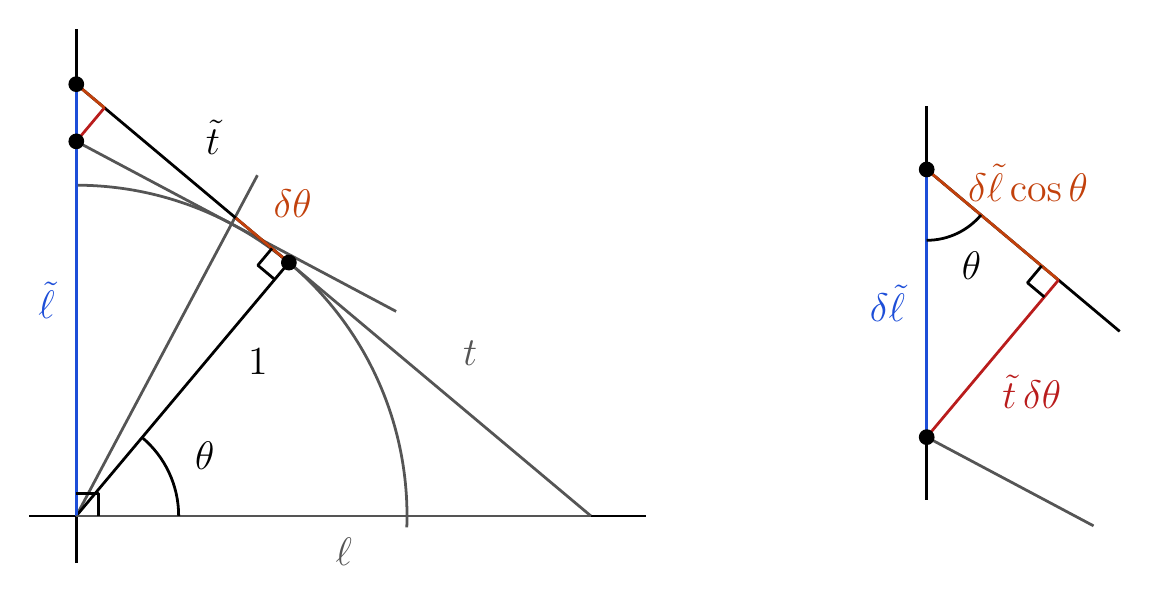
\begin{tikzpicture}[x=1mm, y=1mm]
  \def\U{42}\def\Th{50}\def\dTh{12}     % radius (= 1), angle, angular nudge

  \pgfmathsetmacro{\Cy}{\U/sin(\Th)}            % c = csc(theta)
  \pgfmathsetmacro{\Xx}{\U/cos(\Th)}            % L = sec(theta)
  \pgfmathsetmacro{\Cyp}{\U/sin(\Th+\dTh)}      % c after the nudge
  \pgfmathsetmacro{\Nrm}{\Th}                   % outward normal of the tangent line
                                                % (the radius direction, of course)
  \pgfmathsetmacro{\Tdir}{\Th-90}               % direction of the tangent line
  \pgfmathsetmacro{\Dcs}{\Cy-\Cyp}              % how far the intercept drops

  \coordinate (O)  at (0,0);
  \coordinate (P)  at (\Th:\U);
  \coordinate (C)  at (0,\Cy);
  \coordinate (Cp) at (0,\Cyp);
  \coordinate (X)  at (\Xx,0);
  % foot of the perpendicular from the nudged intercept onto the line: the
  % third corner of the triangle the right panel magnifies
  \coordinate (Fa) at ({\Dcs*cos(\Th)*cos(\Tdir)},{\Cy+\Dcs*cos(\Th)*sin(\Tdir)});

  % ---------- left: one line cutting both axes --------------------------------
  \draw[hair, muted] (-2:\U) arc[start angle=-2, end angle=90, radius=\U];
  \draw[hair, ink] (-6,0) -- ({\Xx+7},0);
  \draw[hair, ink] (0,-6) -- (0,{\Cy+7});

  % the nudged radius and its tangent line, with the arc between the contacts
  \draw[hair, muted] (O) -- ({\Th+\dTh}:{\U+7});
  \draw[hair, muted] (Cp) -- ++({\Th+\dTh-90}:46);

  \draw[edge, ink]     (O) -- (P);      % the radius, length 1
  \draw[edge, ink]     (C) -- (P);      % r = cot(theta)
  \draw[edge, muted]   (P) -- (X);      % t = tan(theta)
  \draw[edge, figblue] (O) -- (C);      % c = csc(theta)
  \draw[edge, muted]   (O) -- (X);      % L = sec(theta)
  \draw[edge, figred]  (Cp) -- (Fa);    % the leg the right panel calls r*dtheta
  % ORANGE = the two bites taken out of the cotangent leg. At the contact point
  % it slides forward ALONG the line by the arc it travels (drawn straight, not
  % as the arc: near P the two coincide, so an arc here reads as a smudge); at
  % the intercept it gives up the third leg of the small triangle.
  \draw[edge, figorange] (P) -- ++({\Th+90}:{\U*\dTh*pi/180});
  \draw[edge, figorange] (C) -- (Fa);
  \fill[ink] (P) circle (1);
  \fill[ink] (C) circle (1);
  \fill[ink] (Cp) circle (1);

  \draw[hair, ink] (P) ++({\Th+180}:2.8) -- ++({\Th+90}:2.8) -- ++(\Th:2.8);
  \draw[hair, ink] (O) ++(2.8,0) -- ++(0,2.8) -- ++(-2.8,0);

  \draw[hair, ink] (0:13) arc[start angle=0, end angle=\Th, radius=13];
  \node[ink] at ({\Th/2}:18) {$\theta$};
  \node[ink] at ({\Th-9.7}:{0.72*\U}) {$1$};
  \node[text=figorange] at ({\U*cos(\Th)+0.5*\U*\dTh*pi/180*cos(\Th+90)+6*cos(\Nrm)},%
                            {\U*sin(\Th)+0.5*\U*\dTh*pi/180*sin(\Th+90)+6*sin(\Nrm)}) {$\delta\theta$};
  % side labels: each pushed off its own segment along the shared normal
  \node[ink]        at ({0.5*\U*cos(\Th)+6*cos(\Nrm)},{0.5*(\Cy+\U*sin(\Th))+6*sin(\Nrm)}) {$\tilde{t}$};
  \node[text=muted] at ({0.5*(\U*cos(\Th)+\Xx)+6*cos(\Nrm)},{0.5*\U*sin(\Th)+6*sin(\Nrm)}) {$t$};
  \node[left, text=figblue] at (-1.5,{\Cy/2}) {$\tilde{\ell}$};
  \node[below, text=muted]  at ({0.52*\Xx},-1.5) {$\ell$};

  % ---------- right: the corner at C, magnified -------------------------------
  \def\Bx{108}\def\By{44}\def\Dc{34}    % C in the blow-up, and the magnified dc

  \pgfmathsetmacro{\Fbx}{\Bx+\Dc*cos(\Th)*cos(\Tdir)}
  \pgfmathsetmacro{\Fby}{\By+\Dc*cos(\Th)*sin(\Tdir)}

  \coordinate (Cb)  at (\Bx,\By);
  \coordinate (Cpb) at (\Bx,{\By-\Dc});
  \coordinate (Fb)  at (\Fbx,\Fby);

  \draw[hair, ink]   (\Bx,{\By+8}) -- (\Bx,{\By-\Dc-8});     % the y axis
  \draw[hair, muted] (Cpb) -- ++({\Th+\dTh-90}:24);          % the nudged line
  \draw[edge, ink]     (Cb) -- ++(\Tdir:32);                 % on toward P
  \draw[edge, figorange] (Cb) -- (Fb);
  \draw[edge, figred]  (Cpb) -- (Fb);
  \draw[edge, figblue] (Cb) -- (Cpb);
  \fill[ink] (Cb) circle (1);
  \fill[ink] (Cpb) circle (1);

  \draw[hair, ink] (Fb) ++({\Th+180}:2.8) -- ++({\Th+90}:2.8) -- ++(\Th:2.8);

  \draw[hair, ink] ([shift=(270:9)]Cb) arc[start angle=270, end angle={270+\Th}, radius=9];
  \node[ink] at ([shift={({270+\Th/2}:13.5)}]Cb) {$\theta$};
  \node[left, text=figblue] at ({\Bx-1.5},{\By-\Dc/2}) {$\delta\tilde{\ell}$};
  \node[text=figred] at ({0.5*(\Bx+\Fbx)+6.5*cos(\Tdir)},{0.5*(\By-\Dc+\Fby)+6.5*sin(\Tdir)}) {$\tilde{t}\,\delta\theta$};
  \node[text=figorange] at ({0.5*(\Bx+\Fbx)+7*cos(\Nrm)},{0.5*(\By+\Fby)+7*sin(\Nrm)}) {$\delta\tilde{\ell}\cos\theta$};
\end{tikzpicture}
\end{document}
